\documentclass[12pt,a4paper]{article}

\usepackage[T2A]{fontenc}
\usepackage[utf8]{inputenc}
\usepackage[russian]{babel}

\usepackage[left=3cm, right=1.5cm, top=2cm, bottom=2cm]{geometry}

\usepackage{graphicx}
\usepackage{booktabs}
\usepackage{array}
\usepackage{multirow}
\usepackage{float}

\usepackage{amsmath}
\usepackage{amssymb}

\usepackage{hyperref}
\hypersetup{
  colorlinks=true,
  linkcolor=blue,
  citecolor=blue,
  urlcolor=blue
}

\usepackage{cite}

\usepackage{listings}
\lstset{
  basicstyle=\ttfamily\small,
  breaklines=true,
  frame=single,
  language=bash,
  extendedchars=true,
  inputencoding=utf8
}

\usepackage{caption}
\captionsetup{justification=centering}

\usepackage{setspace}
\onehalfspacing

\begin{document}

\begin{titlepage}
  \centering
  \textbf{Российский университет дружбы народов}\\
  \vspace{0.5cm}
  Факультет физико-математических и естественных наук\\
  \vspace{2cm}

  {\Large\bfseries Сравнительный анализ алгоритмов активного управления очередями: RED, ARED, Gentle~RED}\\

  \vspace{3cm}
  \begin{flushright}
    \textbf{Выполнил:}\\
    Палагашвили Абули Михайлович\\
    аспирант\\
    ORCID: 0009-0007-7009-7038\\
    E-mail: 1042250185@rudn.ru\\
  \end{flushright}

  \vfill
  Москва~--- 2026
\end{titlepage}

\setcounter{page}{1}
\tableofcontents
\newpage

\section{Введение}
\label{sec:intro}

Традиционный подход к управлению перегрузкой в маршрутизаторах~--- дроп хвоста (tail-drop): пакеты отбрасываются только тогда, когда буфер полностью заполнен. Это приводит к глобальной синхронизации TCP-потоков, резким осцилляциям пропускной способности и постоянно переполненному буферу. Алгоритмы активного управления очередями (AQM, Active Queue Management) решают эту проблему, начиная отбрасывать или помечать пакеты \textit{заблаговременно}~--- до того, как буфер переполнится~--- на основании статистики средней длины очереди. TCP-соединения получают сигнал о перегрузке раньше и плавнее снижают скорость отправки, не доводя ситуацию до коллапса.

\subsection{RED (Random Early Detection)}

RED~--- базовый алгоритм AQM, предложенный Флойдом и Якобсоном в 1993~году. Алгоритм вычисляет экспоненциально взвешенное скользящее среднее длины очереди (EWMA) и принимает решение о сбросе на его основе.

\textbf{Обновление средней очереди} при каждом поступающем пакете:
\begin{equation}
\bar{q} = (1 - w_q)\,\bar{q} + w_q\,q
\end{equation}
где $q$~--- текущая (мгновенная) длина очереди, $w_q \in (0,1)$~--- вес фильтра.

\textbf{Вероятность сброса} определяется тремя зонами:
\begin{equation}
p(\bar{q}) = \begin{cases}
0 & \bar{q} < \mathrm{min}_{\mathrm{Th}} \\
\mathrm{maxP} \cdot \dfrac{\bar{q} - \mathrm{min}_{\mathrm{Th}}}{\mathrm{max}_{\mathrm{Th}} - \mathrm{min}_{\mathrm{Th}}} & \mathrm{min}_{\mathrm{Th}} \le \bar{q} < \mathrm{max}_{\mathrm{Th}} \\
1 & \bar{q} \ge \mathrm{max}_{\mathrm{Th}}
\end{cases}
\end{equation}

Жёсткий принудительный сброс выше $\mathrm{max}_{\mathrm{Th}}$ обеспечивает быстрое реагирование, но синхронизирует TCP-потоки и создаёт пилообразные осцилляции очереди.

\subsection{ARED (Adaptive RED)}

ARED расширяет RED адаптивным механизмом: параметр $\mathrm{maxP}$ периодически пересчитывается через каждые $T_{\mathrm{interval}}$ в зависимости от отклонения средней очереди от целевого диапазона:
\begin{equation}
\mathrm{maxP} = \begin{cases}
\mathrm{maxP} + \alpha & \bar{q} > \dfrac{\mathrm{min}_{\mathrm{Th}} + \mathrm{max}_{\mathrm{Th}}}{2} \\[6pt]
\mathrm{maxP} - \beta & \bar{q} < \dfrac{\mathrm{min}_{\mathrm{Th}} + \mathrm{max}_{\mathrm{Th}}}{2}
\end{cases}
\end{equation}
где $\alpha$ и $\beta$~--- коэффициенты увеличения и снижения вероятности ($\alpha > \beta$). Значение $\mathrm{maxP}$ ограничивается допустимым диапазоном. Это позволяет алгоритму приспосабливаться к меняющейся нагрузке без ручной настройки, однако адаптация вносит дополнительную инерцию и может приводить к широким колебаниям очереди.

\subsection{Gentle RED}

Gentle RED модифицирует поведение RED в зоне выше $\mathrm{max}_{\mathrm{Th}}$: вместо немедленного принудительного сброса алгоритм продолжает вероятностный подход вплоть до $2 \cdot \mathrm{max}_{\mathrm{Th}}$:
\begin{equation}
p(\bar{q}) = \begin{cases}
0 & \bar{q} < \mathrm{min}_{\mathrm{Th}} \\[4pt]
\mathrm{maxP} \cdot \dfrac{\bar{q} - \mathrm{min}_{\mathrm{Th}}}{\mathrm{max}_{\mathrm{Th}} - \mathrm{min}_{\mathrm{Th}}}
  & \mathrm{min}_{\mathrm{Th}} \le \bar{q} < \mathrm{max}_{\mathrm{Th}} \\[8pt]
\mathrm{maxP} + (1 - \mathrm{maxP}) \cdot \dfrac{\bar{q} - \mathrm{max}_{\mathrm{Th}}}{\mathrm{max}_{\mathrm{Th}}}
  & \mathrm{max}_{\mathrm{Th}} \le \bar{q} < 2\,\mathrm{max}_{\mathrm{Th}} \\[4pt]
1 & \bar{q} \ge 2\,\mathrm{max}_{\mathrm{Th}}
\end{cases}
\end{equation}

В зоне $[\mathrm{max}_{\mathrm{Th}},\, 2\cdot\mathrm{max}_{\mathrm{Th}})$ вероятность линейно растёт от $\mathrm{maxP}$ до~$1$, а принудительный сброс происходит лишь при $\bar{q} \ge 2\cdot\mathrm{max}_{\mathrm{Th}}$. Это смягчает реакцию на кратковременные всплески, снижает синхронизацию TCP-потоков и уменьшает среднюю длину очереди~--- ценой несколько большей вариабельности пропускной способности.

\section{Методы}
\label{sec:methods}

\subsection{Топология эксперимента}

В эксперименте используется топология типа <<гантель>> (dumbbell): несколько отправителей подключены к общему маршрутизатору через быстрые каналы, а маршрутизатор соединён с единственным получателем через узкий канал с ограниченной пропускной способностью. Узкий канал является единственным местом возможной перегрузки, и именно на его исходящем интерфейсе устанавливается дисциплина очереди AQM.

\begin{verbatim}
  Sender 0  --\
  Sender 1  --|
  Sender 2  --|  1 Mbit/s         2 Mbit/s
      ...     |----------> [Router] ----------> Receiver
  Sender 8  --|  delay 2 ms      delay 10 ms
  Sender 9  --/                ^
                          AQM queue
                       (RED / ARED / Gentle)
\end{verbatim}

Каждый из десяти отправителей устанавливает одно TCP-соединение с получателем и непрерывно передаёт данные (BulkSend). Суммарная входящая нагрузка на маршрутизатор потенциально достигает $10 \times 1$~Мбит/с~$= 10$~Мбит/с, что в 5~раз превышает пропускную способность узкого канала. Это обеспечивает устойчивую перегрузку и позволяет оценить поведение алгоритмов AQM в реальных условиях насыщения буфера.

Параметры топологии приведены в табл.~\ref{tab:topology}.

\begin{table}[H]
\centering
\caption{Параметры топологии и симуляции}
\label{tab:topology}
\begin{tabular}{lll}
\toprule
Параметр & Значение & Описание \\
\midrule
\texttt{nSenders} & 10 & Количество TCP-отправителей \\
\texttt{fastRate} & 1 Мбит/с & Скорость каналов отправитель $\to$ маршрутизатор (задержка 2~мс) \\
\texttt{bottleneckRate} & 2 Мбит/с & Скорость узкого канала маршрутизатор $\to$ получатель \\
\texttt{bottleneckDelay} & 10 мс & Задержка узкого канала \\
\texttt{simTime} & 60.0 & Длительность симуляции (с) \\
Транспорт & TCP BulkSend & Размер сегмента 512 байт \\
\bottomrule
\end{tabular}
\end{table}

\subsection{Конфигурация AQM}

Все три алгоритма запускаются с одинаковыми пороговыми параметрами (табл.~\ref{tab:aqm-config}).

\begin{table}[H]
\centering
\caption{Единые пороговые параметры для RED, ARED и Gentle RED}
\label{tab:aqm-config}
\begin{tabular}{lll}
\toprule
Параметр & Значение & Описание \\
\midrule
\texttt{minTh} & 5 пакетов & Нижний порог средней очереди~--- ниже него сбросов нет \\
\texttt{maxTh} & 10 пакетов & Верхний порог; выше него RED/ARED сбрасывают все пакеты \\
\texttt{MaxSize} & 100 пакетов & Жёсткий лимит буфера \\
\bottomrule
\end{tabular}
\end{table}

\subsection{Инструментарий}

В работе использовался дискретно-событийный симулятор сетей \textbf{ns-3} версии~3.41. Симуляционные скрипты размещаются в директории \texttt{scratch/}. Для данного эксперимента создана поддиректория со следующей структурой:

\begin{verbatim}
ns-3.41/
+-- scratch/
    +-- red-experiments/
        +-- red.cc
        +-- configs/
        |   +-- red.txt
        |   +-- ared.txt
        |   +-- gentle.txt
        +-- analysis/
            +-- vis.py
            +-- ...
\end{verbatim}

Конфигурационные файлы задают тип AQM и параметры очереди. Пример \texttt{configs/red.txt}:

\begin{lstlisting}
aqmType=red
minTh=5
maxTh=10
MaxSize=100
\end{lstlisting}

Аналогичные файлы для ARED (\texttt{aqmType=ared}) и Gentle RED (\texttt{aqmType=gentle}) отличаются лишь значением поля \texttt{aqmType}.

Симуляции запускались командой:
\begin{lstlisting}
./ns3 run "scratch/red-experiments/red.cc --config=configs/<algorithm>.txt"
\end{lstlisting}

По завершении каждой симуляции три CSV-файла перемещались в директорию \texttt{analysis/}:
\begin{itemize}
  \item \texttt{<algorithm>\_queue.csv}~--- длина очереди раз в 100~мс;
  \item \texttt{<algorithm>\_drops.csv}~--- метки времени каждого сброса пакета;
  \item \texttt{<algorithm>\_throughput.csv}~--- пропускная способность раз в 100~мс.
\end{itemize}

Для построения графиков использовался скрипт \texttt{vis.py} со сглаживанием скользящим средним (окно 30 отсчётов):
\begin{lstlisting}
python vis.py --algorithms red ared gentle --window 30
\end{lstlisting}

\subsection{Метрики оценки}

\begin{table}[H]
\centering
\caption{Метрики оценки алгоритмов}
\label{tab:metrics}
\begin{tabular}{lll}
\toprule
Метрика & Источник данных & Что характеризует \\
\midrule
Средняя и медианная длина очереди & \texttt{*\_queue.csv} & Средняя задержка в буфере \\
p90 / p99 длины очереди & \texttt{*\_queue.csv} & Хвостовые задержки \\
Доля времени с пустой очередью & \texttt{*\_queue.csv} & Недоиспользование канала \\
Средняя пропускная способность & \texttt{*\_throughput.csv} & Утилизация канала \\
Коэффициент вариации (CV) & \texttt{*\_throughput.csv} & Стабильность потока \\
Общее число сбросов & \texttt{*\_drops.csv} & Нагрузка на TCP-механизм перегрузки \\
Медиана интервала между сбросами & \texttt{*\_drops.csv} & Характер управляющих сигналов \\
\bottomrule
\end{tabular}
\end{table}

\section{Результаты}
\label{sec:results}

Эксперимент состоял из трёх последовательных симуляций~--- по одной на каждый алгоритм. Каждый из трёх алгоритмов запускался с одинаковыми параметрами очереди (табл.~\ref{tab:aqm-config}) в течение 60~секунд (первая секунда~--- прогрев, из анализа исключена).

\subsection{Динамика очереди}

На рис.~\ref{fig:queue} представлена динамика длины очереди для трёх алгоритмов за всё время симуляции.

\begin{figure}[H]
\centering
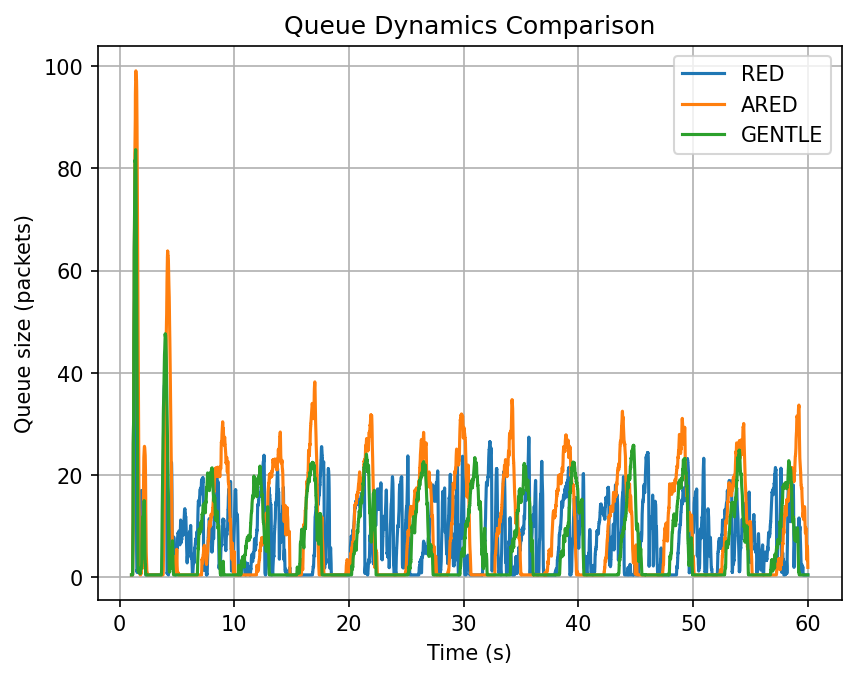
\includegraphics[width=\textwidth]{../queue.png}
\caption{Динамика длины очереди для RED, ARED и Gentle RED}
\label{fig:queue}
\end{figure}

На графике чётко выделяются две фазы.

\textbf{Фаза медленного старта ($t = 0$--$4$~с).} Все TCP-соединения одновременно входят в slow-start и за секунды насыщают буфер. Очередь у всех алгоритмов достигает пиковых значений: ARED~--- до 100~пакетов, RED и Gentle RED~--- до 84~пакетов. Этот выброс одинаков для всех трёх, поскольку алгоритм AQM ещё не успел накопить статистику и среагировать.

\textbf{Установившийся режим ($t > 5$~с).} После рассасывания начального всплеска алгоритмы расходятся в поведении.

\textbf{RED} (синяя кривая) удерживает очередь в диапазоне 5--26~пакетов с относительно регулярными осцилляциями. Кривая редко касается нуля (пустая очередь лишь 13.4\% времени): принудительный сброс при \texttt{m\_qAvg >= maxTh} реагирует быстро и держит очередь <<в узде>>, но ценой постоянного давления на TCP-потоки.

\textbf{ARED} (оранжевая кривая) демонстрирует наибольшую амплитуду колебаний и наиболее хаотичный рисунок. Периодически очередь вырастает до 30--35~пакетов в установившемся режиме и резко обваливается к нулю. Это следствие адаптации $\mathrm{maxP}$: алгоритм поочерёдно <<отпускает>> и <<закручивает>> вероятность сброса, порождая широкие и нерегулярные циклы. p99~$= 49$~пакетов~--- самое высокое значение среди трёх алгоритмов.

\textbf{Gentle RED} (зелёная кривая) чаще остальных возвращается к нулю (26.6\% времени очередь пуста, медиана~$= 1$~пакет). Плавная вероятностная функция в зоне \texttt{[maxTh, 2*maxTh]} позволяет TCP-потокам десинхронизировать свои окна, что приводит к более глубоким, но менее длительным <<провалам>> очереди.

Статистика установившегося режима приведена в табл.~\ref{tab:queue-stats}.

\begin{table}[H]
\centering
\caption{Статистика длины очереди в установившемся режиме}
\label{tab:queue-stats}
\begin{tabular}{lcccccc}
\toprule
Алгоритм & Среднее (пкт) & Стд. откл. & Медиана & p90 & p99 & Пустая (\%) \\
\midrule
RED      & 7.74  & 7.45  & 6 & 18 & 26 & 13.4\% \\
ARED     & 9.57  & 11.94 & 4 & 25 & 49 & 22.3\% \\
Gentle   & 6.40  & 8.86  & 1 & 19 & 34 & 26.6\% \\
\bottomrule
\end{tabular}
\end{table}

Распределение времени по зонам работы EWMA-средней $\bar{q}$ показано в табл.~\ref{tab:zones}.

\begin{table}[H]
\centering
\caption{Доля времени в каждой зоне управления очередью}
\label{tab:zones}
\begin{tabular}{lcccc}
\toprule
Алгоритм & $\bar{q} < \mathrm{min}_{\mathrm{Th}}$ & $[\mathrm{min}_{\mathrm{Th}}, \mathrm{max}_{\mathrm{Th}})$ & $[\mathrm{max}_{\mathrm{Th}}, 2\mathrm{max}_{\mathrm{Th}})$ & $\bar{q} \ge 2\mathrm{max}_{\mathrm{Th}}$ \\
\midrule
RED      & 46.0\% & 19.8\% & 29.3\% & 4.8\%  \\
ARED     & 52.6\% & 8.0\%  & 19.6\% & 19.7\% \\
Gentle   & 60.8\% & 11.8\% & 19.8\% & 7.7\%  \\
\bottomrule
\end{tabular}
\end{table}

RED проводит 34.1\% времени в зоне принудительного сброса (\texttt{m\_qAvg >= maxTh}), что объясняет его высокую среднюю очередь. ARED проводит 19.7\% времени в зоне $\bar{q} \ge 2\cdot\mathrm{max}_{\mathrm{Th}}$, где дропаются все пакеты,~--- отсюда его аномально высокое p99. Gentle RED чаще всего находится ниже minTh (60.8\%) и реже всего попадает в зону жёстких сбросов (7.7\%).

\subsection{Пропускная способность}

График пропускной способности (рис.~\ref{fig:throughput}) построен с применением скользящего среднего с окном 30~отсчётов, поэтому отображает данные начиная с $t \approx 29$~с. Ось~Y намеренно сжата до диапазона 1.74--1.86~Мбит/с, что позволяет рассмотреть различия, невидимые на полной шкале.

\begin{figure}[H]
\centering
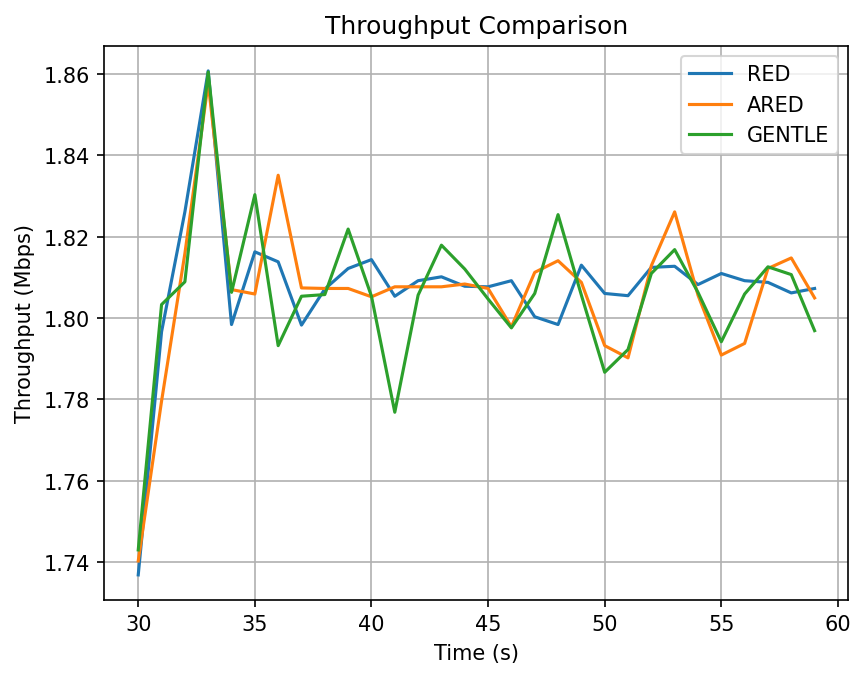
\includegraphics[width=\textwidth]{../throughput.png}
\caption{Пропускная способность: сравнение RED, ARED и Gentle RED}
\label{fig:throughput}
\end{figure}

Все три алгоритма стабильно удерживают пропускную способность вблизи \textbf{1.80--1.81~Мбит/с} ($\sim$90\% от номинала канала 2~Мбит/с). Это означает, что выбор алгоритма AQM при данных параметрах не влияет на утилизацию полосы: все три механизма одинаково эффективно <<заполняют>> канал.

Характерный пик около $t = 33$~с (все кривые достигают $\sim$1.86~Мбит/с)~--- синхронное восстановление TCP-потоков после первоначальной волны сбросов: окна конгестии одновременно начинают расти, создавая кратковременный избыточный поток.

\begin{table}[H]
\centering
\caption{Статистика пропускной способности (CV~--- коэффициент вариации)}
\label{tab:throughput}
\begin{tabular}{lccccc}
\toprule
Алгоритм & Среднее (Мбит/с) & Стд. откл. & Мин. & Макс. & CV \\
\midrule
RED      & 1.8047 & 0.3380 & 0.533 & 3.621 & 18.7\% \\
ARED     & 1.8039 & 0.3950 & 0.553 & 3.293 & 21.9\% \\
Gentle   & 1.7998 & 0.4444 & 0.352 & 3.654 & 24.7\% \\
\bottomrule
\end{tabular}
\end{table}

Несмотря на одинаковое среднее, \textbf{RED демонстрирует наименьшую вариабельность} (CV~$= 18.7\%$): жёсткий синхронный сброс держит все TCP-потоки в такт, делая пропускную способность предсказуемой. Gentle RED имеет наибольший CV (24.7\%)~--- асинхронное управление окнами создаёт большую <<рябь>>, хотя среднее значение от этого не страдает.

\subsection{Сбросы пакетов}

График (рис.~\ref{fig:drops}) представляет моменты сбросов в виде точечной диаграммы: каждая точка~--- один сброшенный пакет. Три горизонтальные полосы соответствуют трём алгоритмам.

\begin{figure}[H]
\centering
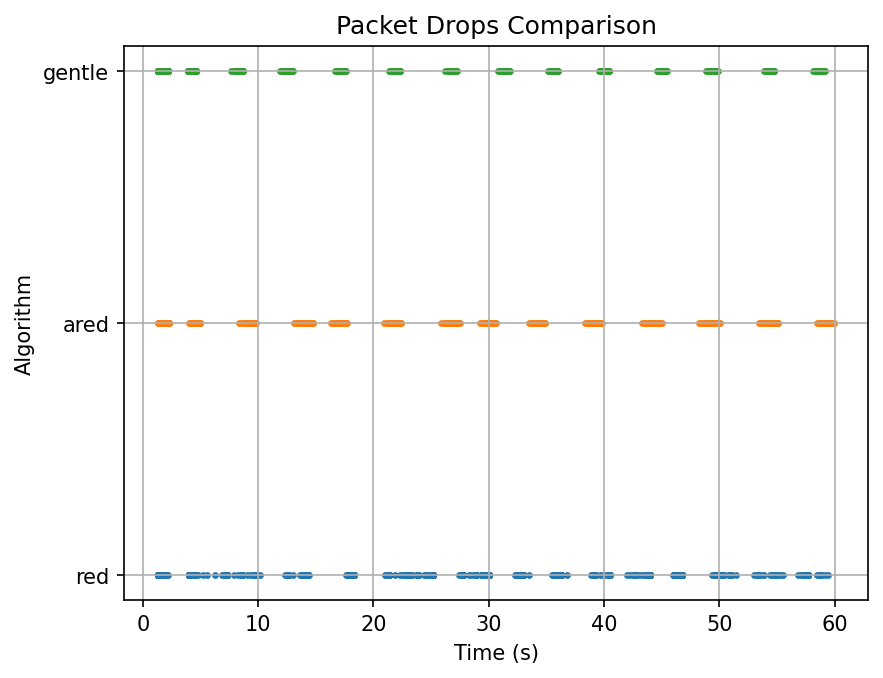
\includegraphics[width=\textwidth]{../drops.png}
\caption{Моменты сбросов пакетов для каждого алгоритма}
\label{fig:drops}
\end{figure}

\textbf{RED} (нижняя полоса, синий)~--- самая плотная и непрерывная полоса: точки заполняют практически всё время симуляции, лишь с редкими небольшими просветами. RED активно дропает в 47 из 58~секунд со средним интервалом между сбросами всего \textbf{2.3~мс} (медиана). Принудительный сброс при \texttt{m\_qAvg >= maxTh} создаёт непрерывный поток отброшенных пакетов каждый раз, как средняя очередь превышает порог.

\textbf{ARED} (средняя полоса, оранжевый)~--- чётко видны кластеры сбросов, разделённые заметными паузами. Алгоритм активен в 33 из 58~секунд. Адаптация $\mathrm{maxP}$ периодически снижает вероятность сброса до нуля, давая потокам <<передышку>>. Однако когда сбросы происходят, их плотность внутри кластера высока (максимальный всплеск~--- 276 сбросов в секунду).

\textbf{Gentle RED} (верхняя полоса, зелёный)~--- наиболее выраженная кластерная структура с самыми длинными паузами между кластерами. Алгоритм активен лишь в 27 из 58~секунд. Внутри каждого кластера сбросы плотные (максимальный всплеск~--- 305/с), однако между ними~--- длительные <<тихие>> промежутки.

Сводная статистика сбросов приведена в табл.~\ref{tab:drops}.

\begin{table}[H]
\centering
\caption{Статистика сбросов пакетов}
\label{tab:drops}
\begin{tabular}{lccccc}
\toprule
Алгоритм & Всего сбросов & Частота (сбр./с) & Медиана интервала & Активных секунд & Макс. всплеск \\
\midrule
RED      & 1240 & 21.34 & 2.3 мс  & 47 & 321 \\
ARED     & 1003 & 17.11 & 11.3 мс & 33 & 276 \\
Gentle   & 1026 & 17.75 & 9.1 мс  & 27 & 305 \\
\bottomrule
\end{tabular}
\end{table}

RED генерирует на \textbf{19--21\% больше сбросов}, чем конкуренты. Медиана интервала между сбросами у RED (2.3~мс) в 4--5~раз меньше, чем у ARED и Gentle,~--- RED практически непрерывно дропает пакеты в периоды перегрузки, тогда как ARED и Gentle работают <<импульсами>>.

\section{Обсуждение}
\label{sec:discussion}

Итоговое сравнение алгоритмов по всем ключевым метрикам представлено в табл.~\ref{tab:summary}.

\begin{table}[H]
\centering
\caption{Сводное сравнение алгоритмов RED, ARED и Gentle RED}
\label{tab:summary}
\begin{tabular}{lccc}
\toprule
Метрика & RED & ARED & Gentle RED \\
\midrule
Средняя пропускная способность & 1.8047 Мбит/с & 1.8039 Мбит/с & 1.7998 Мбит/с \\
CV пропускной способности & \textbf{18.7\%} & 21.9\% & 24.7\% \\
Средняя очередь & 7.74 пкт & 9.57 пкт & \textbf{6.40 пкт} \\
Стд. откл. очереди & 7.45 & 11.94 & 8.86 \\
p99 очереди & 26 пкт & 49 пкт & 34 пкт \\
Пустая очередь (\%) & 13.4\% & 22.3\% & \textbf{26.6\%} \\
Всего сбросов & 1240 & \textbf{1003} & 1026 \\
Характер сбросов & непрерывный & кластерный & импульсный \\
Медиана интервала между сбросами & 2.3 мс & 11.3 мс & 9.1 мс \\
\bottomrule
\end{tabular}
\end{table}

\textbf{RED} обеспечивает наиболее предсказуемую и стабильную пропускную способность (CV~$= 18.7\%$), но достигает этого ценой наибольшего числа сбросов (1240) и наиболее высокой средней очереди. Непрерывный характер сбросов синхронизирует TCP-потоки, создавая жёсткую, <<квантованную>> динамику управления перегрузкой.

\textbf{ARED} минимизирует число сбросов (1003, $-19\%$ к RED) и реже всего тревожит потоки. Однако адаптация $\mathrm{maxP}$ создаёт значительную нестабильность очереди (стд.~$= 11.94$, p99~$= 49$~пакетов) с периодами чрезмерного роста буфера~--- потенциально нежелательными с точки зрения задержки.

\textbf{Gentle RED} достигает наименьшей средней очереди (6.40~пакета) и наибольшей доли пустого буфера (26.6\%). Число сбросов сопоставимо с ARED (1026), однако они распределены наиболее компактными импульсами с длинными паузами между ними. Платой является наибольшая вариабельность пропускной способности (CV~$= 24.7\%$) вследствие десинхронизации TCP-потоков.

\section{Заключение}
\label{sec:conclusion}

Проведённый эксперимент показал, что все три алгоритма AQM~--- RED, ARED и Gentle RED~--- обеспечивают практически одинаковую среднюю пропускную способность ($\sim$1.80~Мбит/с, $\sim$90\% от номинала канала), однако принципиально различаются по характеру управления буфером и нагрузке на механизм управления перегрузкой TCP.

Ключевое различие состоит в компромиссе между предсказуемостью и агрессивностью управления очередью. RED действует наиболее агрессивно: принудительный сброс при превышении $\mathrm{max}_{\mathrm{Th}}$ удерживает очередь <<в узде>> (средняя 7.74~пакета) и обеспечивает минимальную вариабельность пропускной способности (CV~$= 18.7\%$), но ценой наибольшего числа сбросов (1240) и непрерывного давления на TCP-потоки. ARED, напротив, жертвует стабильностью очереди ради снижения числа сбросов: адаптация $\mathrm{maxP}$ уменьшает сбросы на 19\% по сравнению с RED, однако порождает широкие осцилляции (стд.~$= 11.94$, p99~$= 49$~пакетов), неприемлемые для приложений, чувствительных к задержке. Gentle RED занимает промежуточное положение, достигая наименьшей средней очереди (6.40~пакета) за счёт более плавной функции сброса, которая десинхронизирует TCP-потоки и снижает заполненность буфера,~--- но при этом увеличивает вариабельность пропускной способности (CV~$= 24.7\%$).

Полученные результаты подтверждают, что выбор алгоритма AQM определяется требованиями конкретного сценария: не существует единственного <<лучшего>> решения~--- каждый алгоритм оптимален по своей целевой метрике.

\textbf{Рекомендации по применению:}
\begin{itemize}
  \item При приоритете \textbf{минимальной задержки в буфере}~--- Gentle RED (наименьшая средняя очередь 6.40~пкт).
  \item При приоритете \textbf{минимального числа сбросов}~--- ARED (на 19\% меньше сбросов, чем RED).
  \item При приоритете \textbf{предсказуемой пропускной способности}~--- RED (наименьший CV 18.7\%).
\end{itemize}

\end{document}
